\documentclass{beamer}

% \usepackage{beamerthemesplit} // Activate for custom appearance

\title{Math 493 Project 2}
\author{Aneesh \& JJ \& Matt}
\date{\today}

\begin{document}

\frame{\titlepage}

\section[Outline]{}

\section{Problem 1}


\frame{
\frametitle{Trajectory Matching with Markov Chain Monte Carlo}

Since the ODE function given could be easily solved, the problem became estimating $C$ and $\beta$ in $Ce^{-\beta t}$.\\
We first initialized the Markov Chain Monte Carlo with the following parameters:\\
\begin{center}
\begin{tabular}{|c|c|}
\hline
Variable & Value\\
\hline
$C_0$ & 0\\
$\beta_0$ & 0\\
Data Standard Deviation $\sigma$ & 0.03\\
Guess Jump & 0.01\\
Burn Time & 100\\
Iteration Limit & 5000\\
\hline
\end{tabular}
\end{center}
}

\frame{
\frametitle{Trajectory Matching with Markov Chain Monte Carlo}

For each iteration step:
\begin{enumerate}
\item make a new guess for $[C_n,\beta_n]=[C_{n-1},\beta_{n-1}]+D*\text{randn}$
\item calculate the SSE using $[C_n,\beta_n]$
\item evaluate the ratio $e^{\frac{-\text{SSE}_{n-1}+\text{SSE}_n}{2\sigma^2}}$
\item if a random number between 0 and 1 is smaller than the ratio, the new guess is accepted
\end{enumerate}
}

\frame{
\frametitle{Trajectory Matching with Markov Chain Monte Carlo}
With the smoother version of the data, we obtained the following result:
\begin{center}
\begin{tabular}{|cc|}
\hline
C & 3.1792\\
\hline
$\beta$ & 5.5447\\
\hline
\end{tabular}
\end{center}
}

\frame{
\frametitle{Trajectory Matching with Markov Chain Monte Carlo}
We can also observe the convergence in the following figure:
\begin{figure}[H]
\centering
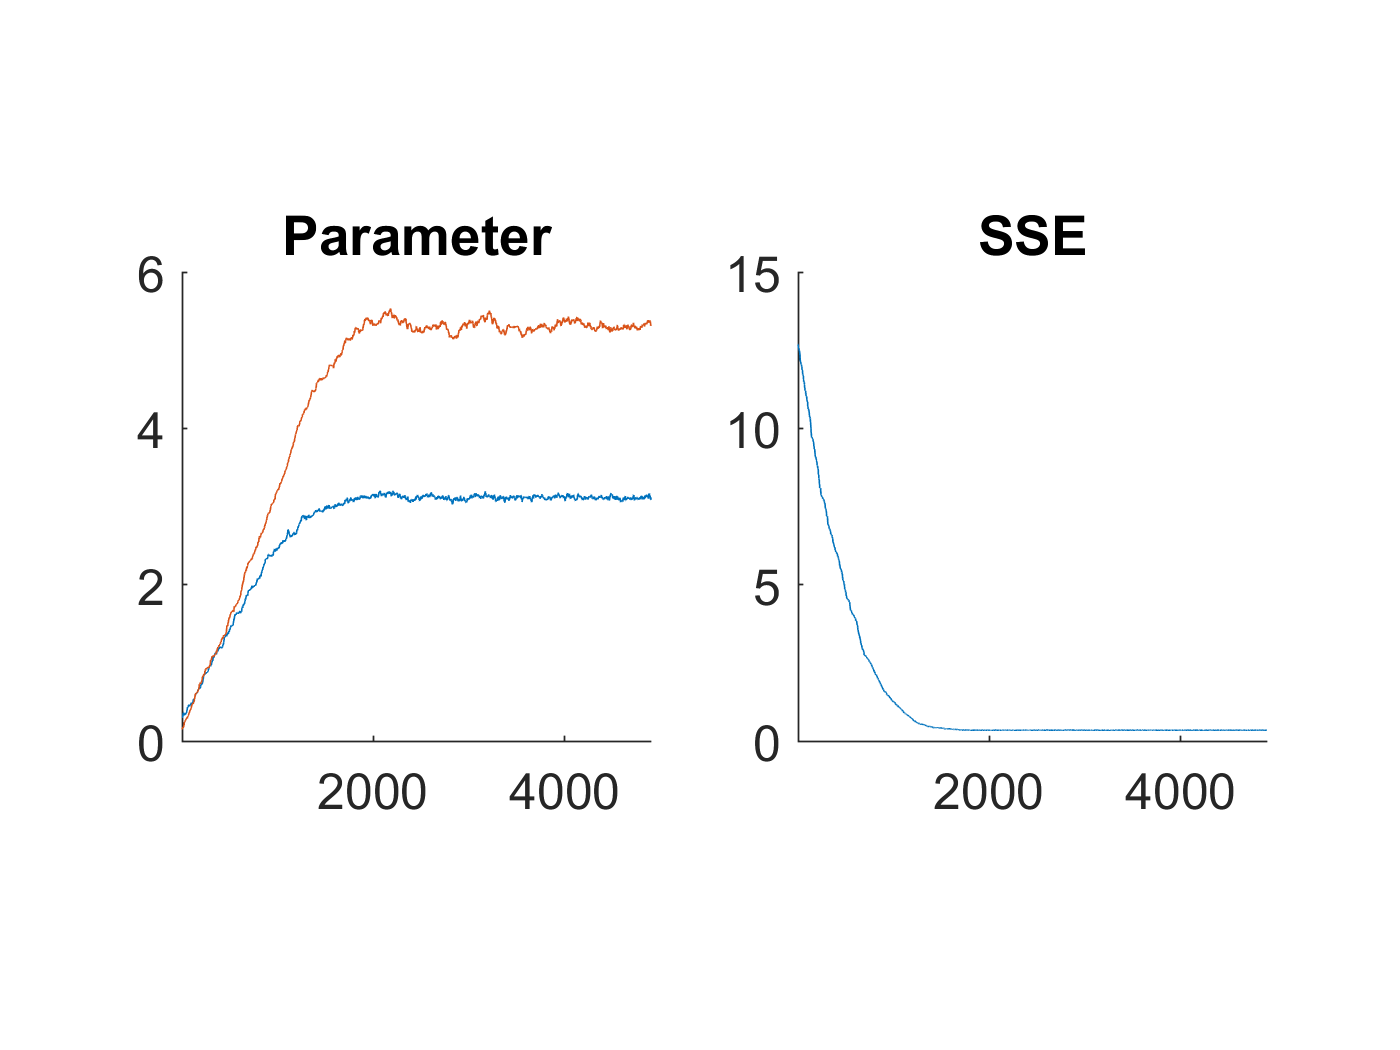
\includegraphics[scale=0.2]{figures/p_a_conv.png}
\end{figure}
}

\frame{
\frametitle{Trajectory Matching with Markov Chain Monte Carlo}

We can also see how our model compares with the data:
\begin{figure}[H]
\centering
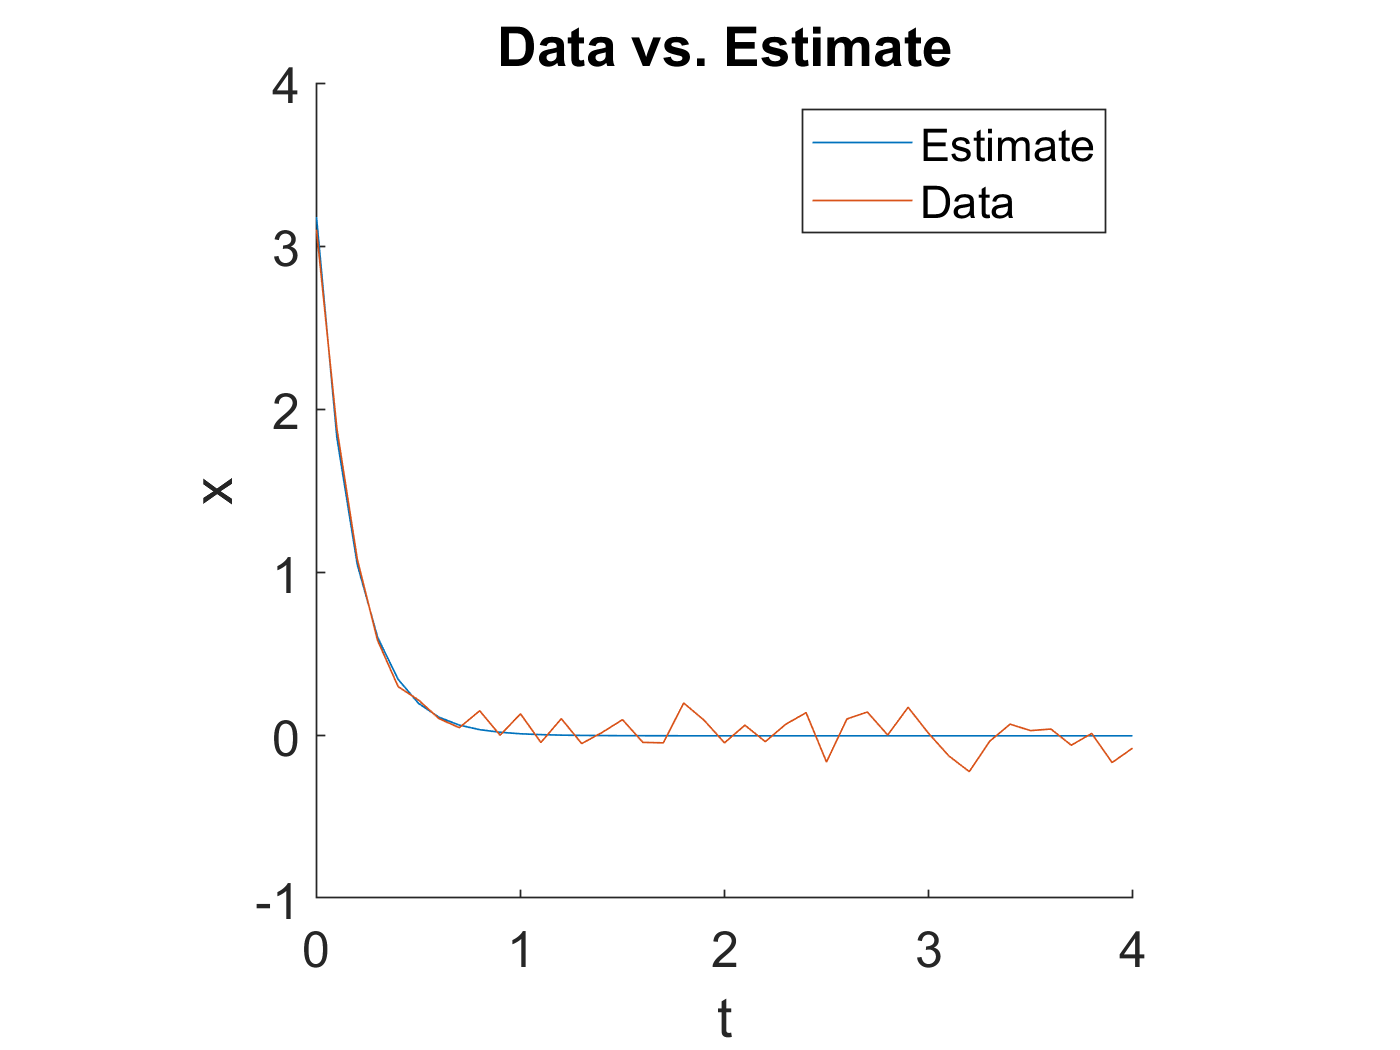
\includegraphics[scale=0.2]{figures/p_a_data.png}
\end{figure}

}

\frame{
\frametitle{Trajectory Matching with Markov Chain Monte Carlo}

With the noisy version of the data, we obtained the following result:
\begin{center}
\begin{tabular}{|c|c|}
\hline
C & 2.6331\\
\hline
$\beta$ & 4.8364\\
\hline
\end{tabular}
\end{center}
}

\frame{
\frametitle{Trajectory Matching with Markov Chain Monte Carlo}

We can also observe the convergence in the following figure:
\begin{figure}[H]
\centering
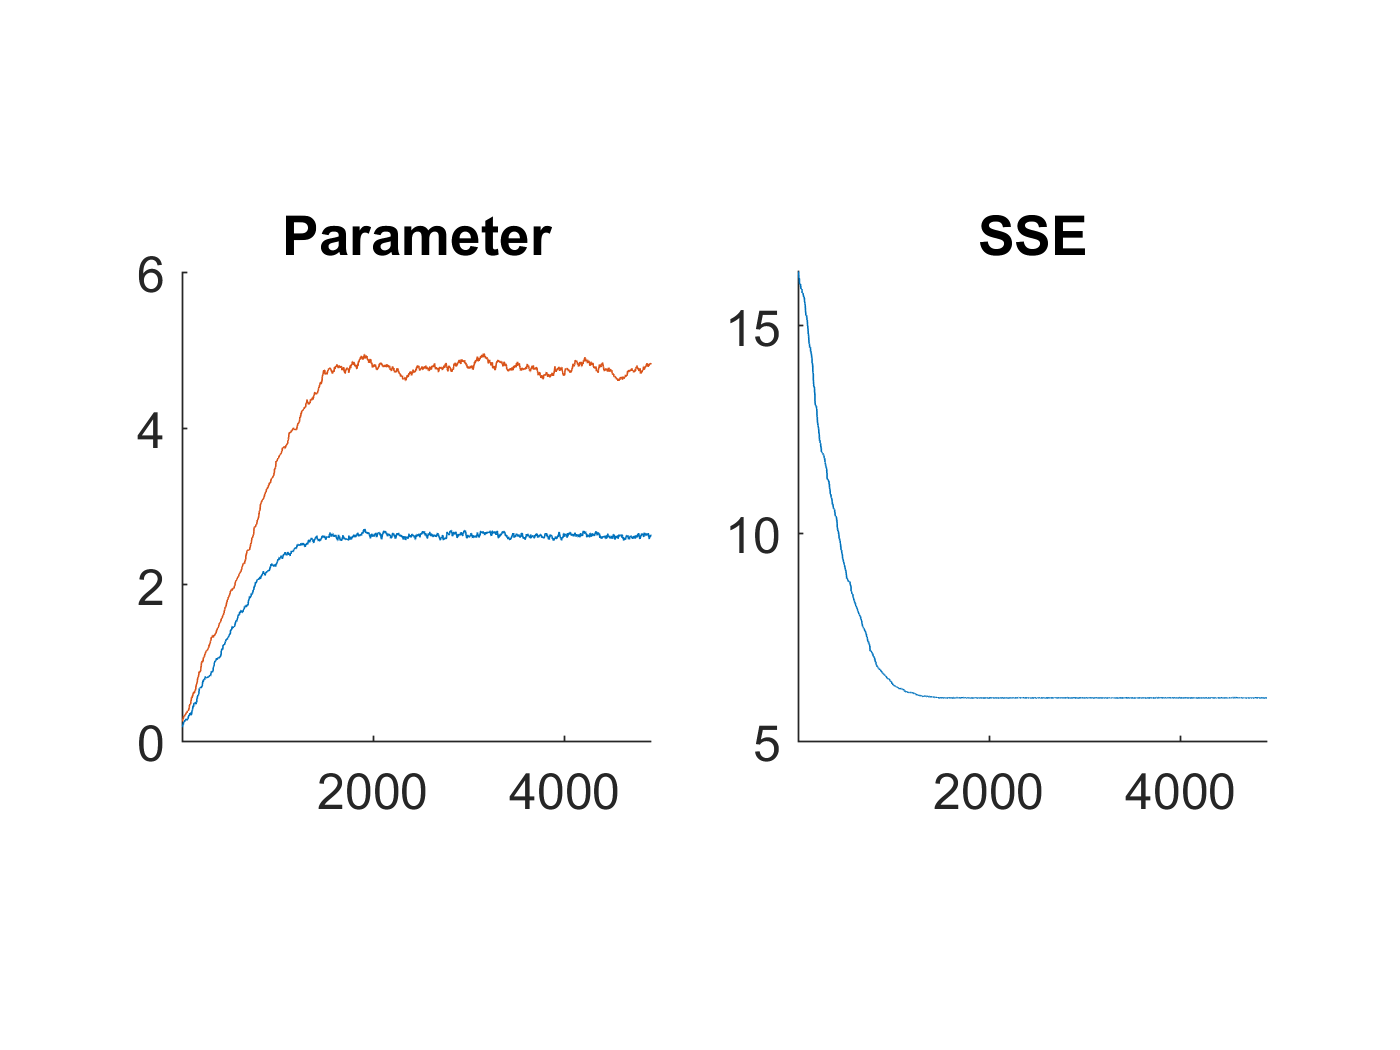
\includegraphics[scale=0.2]{figures/p_a_conv_1.png}
\end{figure}
}

\frame{
\frametitle{Trajectory Matching with Markov Chain Monte Carlo}

We can also see how our model compares with the data:
\begin{figure}[H]
\centering
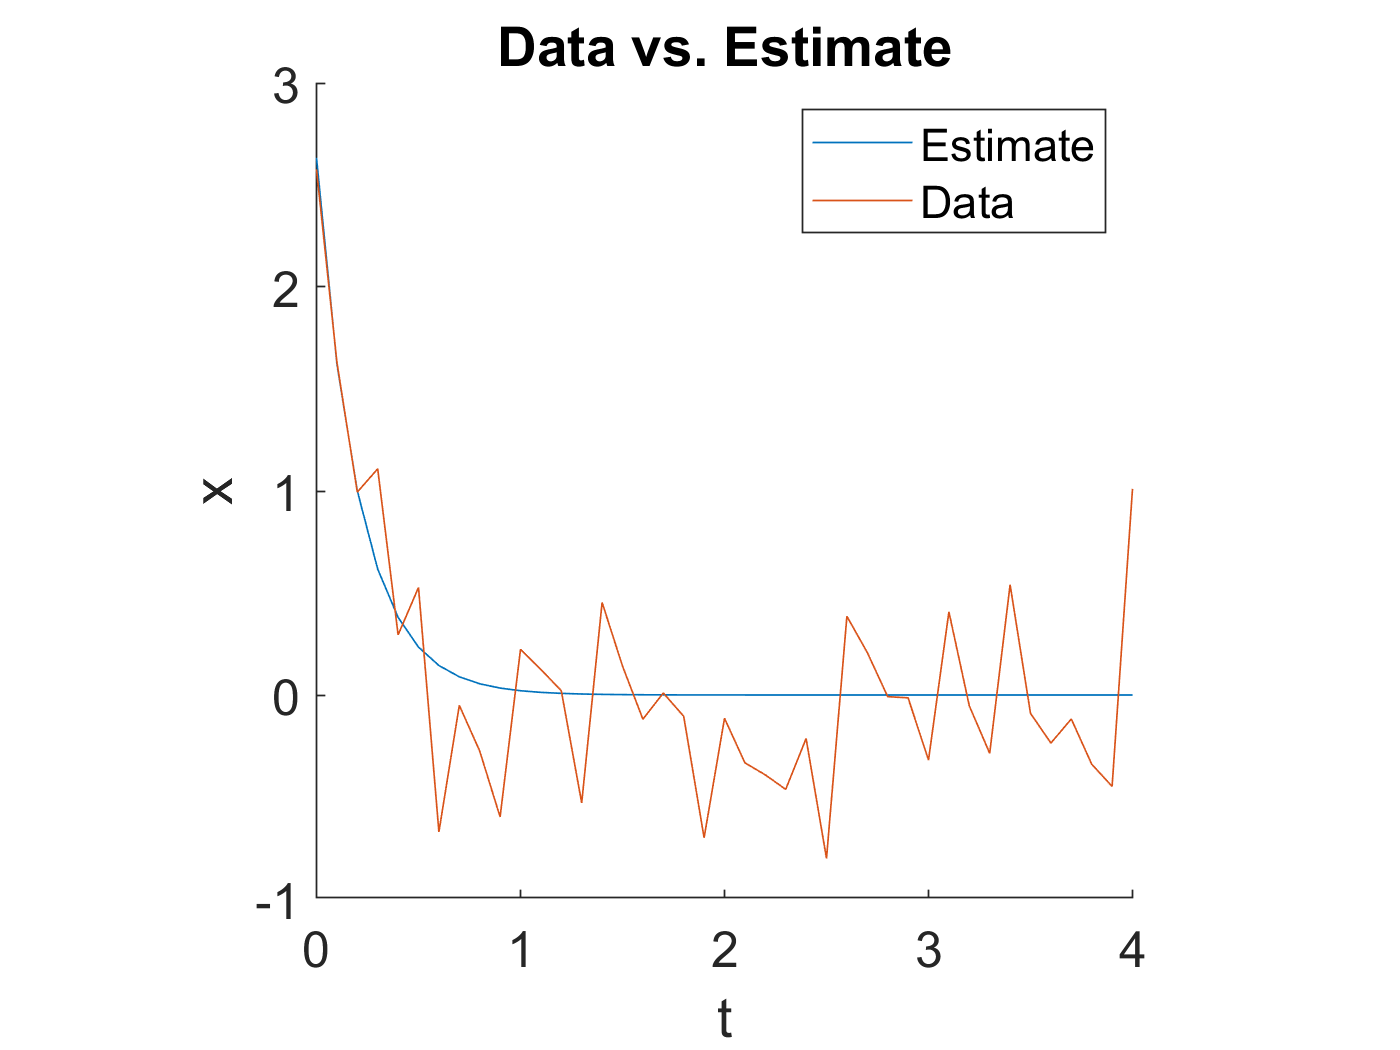
\includegraphics[scale=0.2]{figures/p_a_data_1.png}
\end{figure}

}

\frame{
\frametitle{Trajectory Matching with Markov Chain Monte Carlo}
We explored with the guess jump a little bit and obtained the following result:
\begin{center}
\begin{tabular}{|c|c|c|c|c|}
\hline
Guess Jump & C & $\beta$ & Converged Step& Converged SSE\\
\hline
0.005 & 3.1656 & 5.4653 & 4326 & 0.3466\\
0.01 & 3.1200 & 5.3525 & 2073	 & 0.3446\\
0.02 & 3.0976 & 5.2793 & 755 & 0.3458\\
0.1 & 3.1783 & 5.5051 & 99 & 0.3482\\
\hline
\end{tabular}
\end{center}
}

\frame{
\frametitle{Gradient Matching with Smoothing}
We can smooth the data using collocation. The basis $\phi$ could be created using \textit{spcol} function in matlab. Then the coefficients $\mathbf{c}=(\phi^{T}\phi)^{-1}(\phi y)$, where $y$ is the data given.\\

The gradient matching method is essentially using Gauss-Newton method to minimize the integrated SSE:
$$\text{ISSE}=\sum_{i=1}^n W_{i} [D\hat{x(t_i)}-f(\hat{x(t_i)},\theta)]^2$$
where $\hat{x(t_i)}=\phi \mathbf{c}$ is the smoothed data using collocation. \\
For this problem, the ISSE could be simplied to 
$$\text{ISSE}=\sum_{i=1}^n W_{i} [D\phi(t_i)\mathbf{c}+\beta \phi(t_i)\mathbf{c}]^2$$
}

\frame{
\frametitle{Gradient Matching with Smoothing}
Then the Jacobian becomes $\hat{x}$. For each iteration step, we perform the following:
\begin{center}
\begin{equation}
\begin{split}
H & = J^{T}J\\
g & = J^{T}(D\hat{x}+\beta\hat{x})\\
\beta_n & = \beta_{n-1} - H^{-1}g
\end{split}
\end{equation}
\end{center}
Due to the fact that ISSE does not take $x(t_0)$ into account, we use the initial value of the smoothed data as $x(t_0)$ for the following parts.
}

\frame{
\frametitle{Gradient Matching with Smoothing}
With the smoother version of the data, the estimated $\beta=4.962410410929266$.\\
We can also observe the convergence in the following figure:
\begin{figure}[H]
\centering
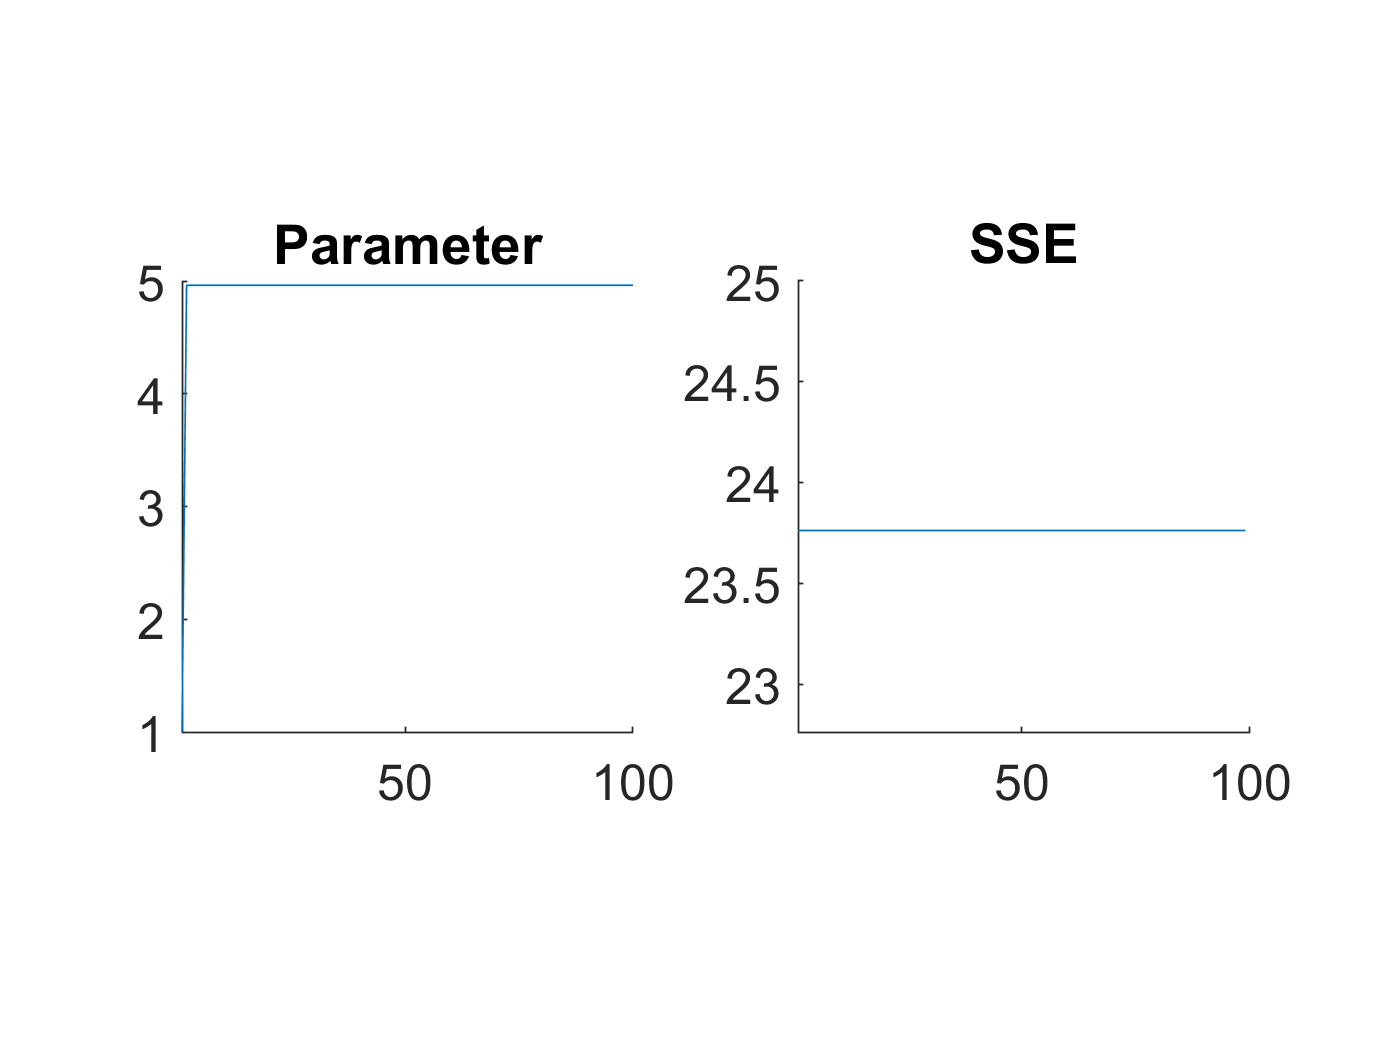
\includegraphics[scale=0.25]{figures/p_b_conv.png}
\end{figure}
}

\frame{
\frametitle{Gradient Matching with Smoothing}
We can also see how our model compares with the data:
\begin{figure}[H]
\centering
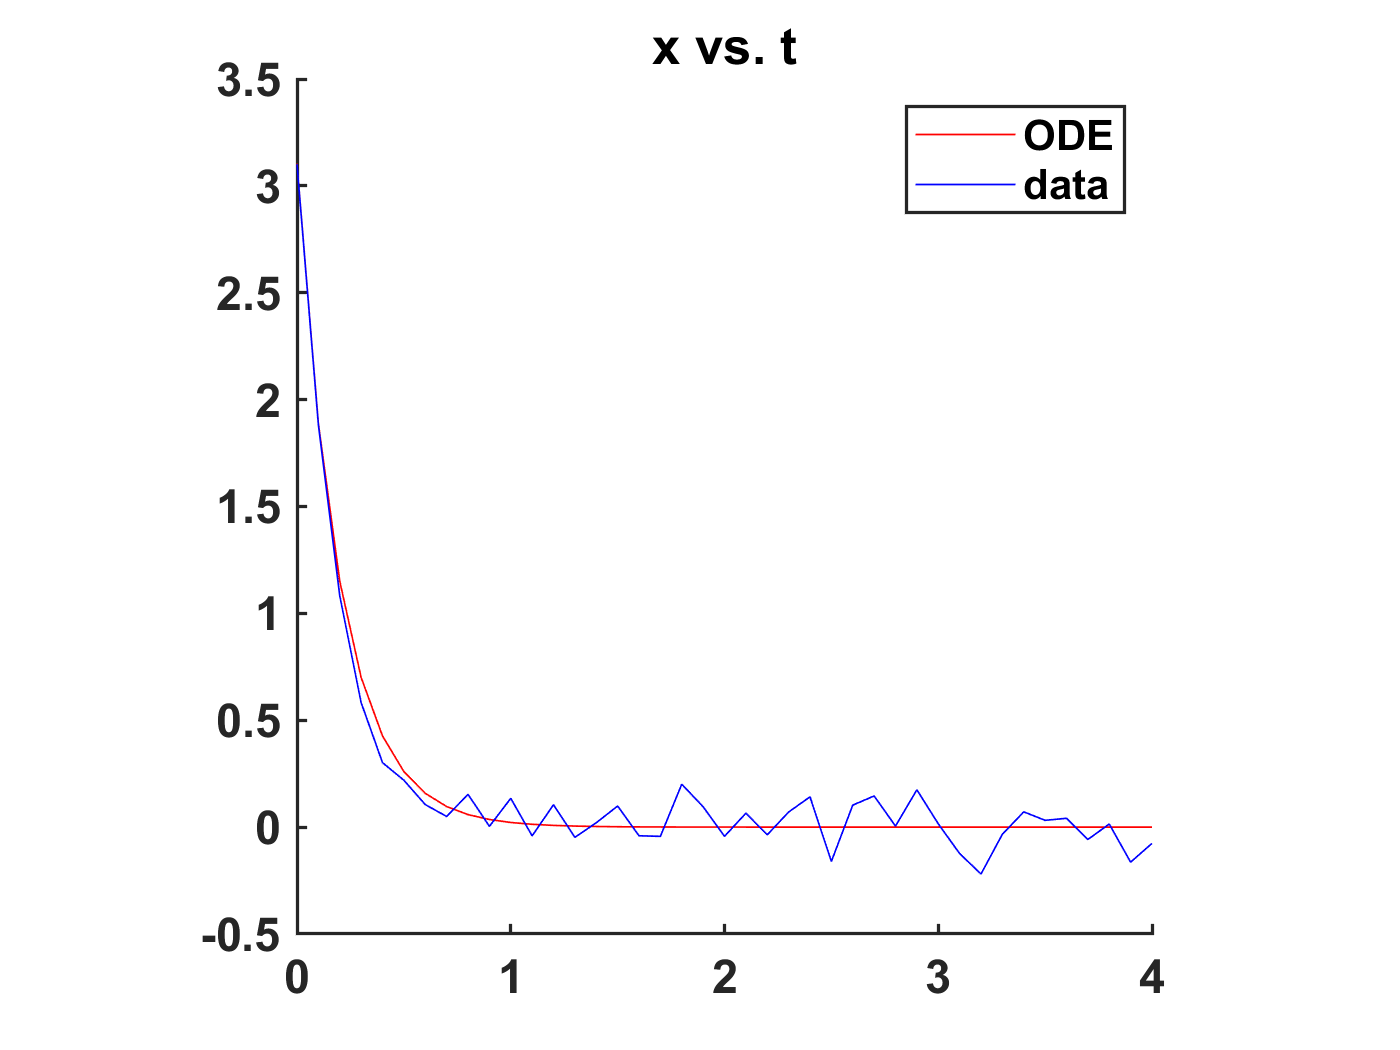
\includegraphics[scale=0.2]{figures/p_b_data.png}
\end{figure}
}

\frame{
\frametitle{Gradient Matching with Smoothing}
With the noisy version of the data, the estimated $\beta=2.160787567688269$.\\
We can also observe the convergence in the following figure:
\begin{figure}[H]
\centering
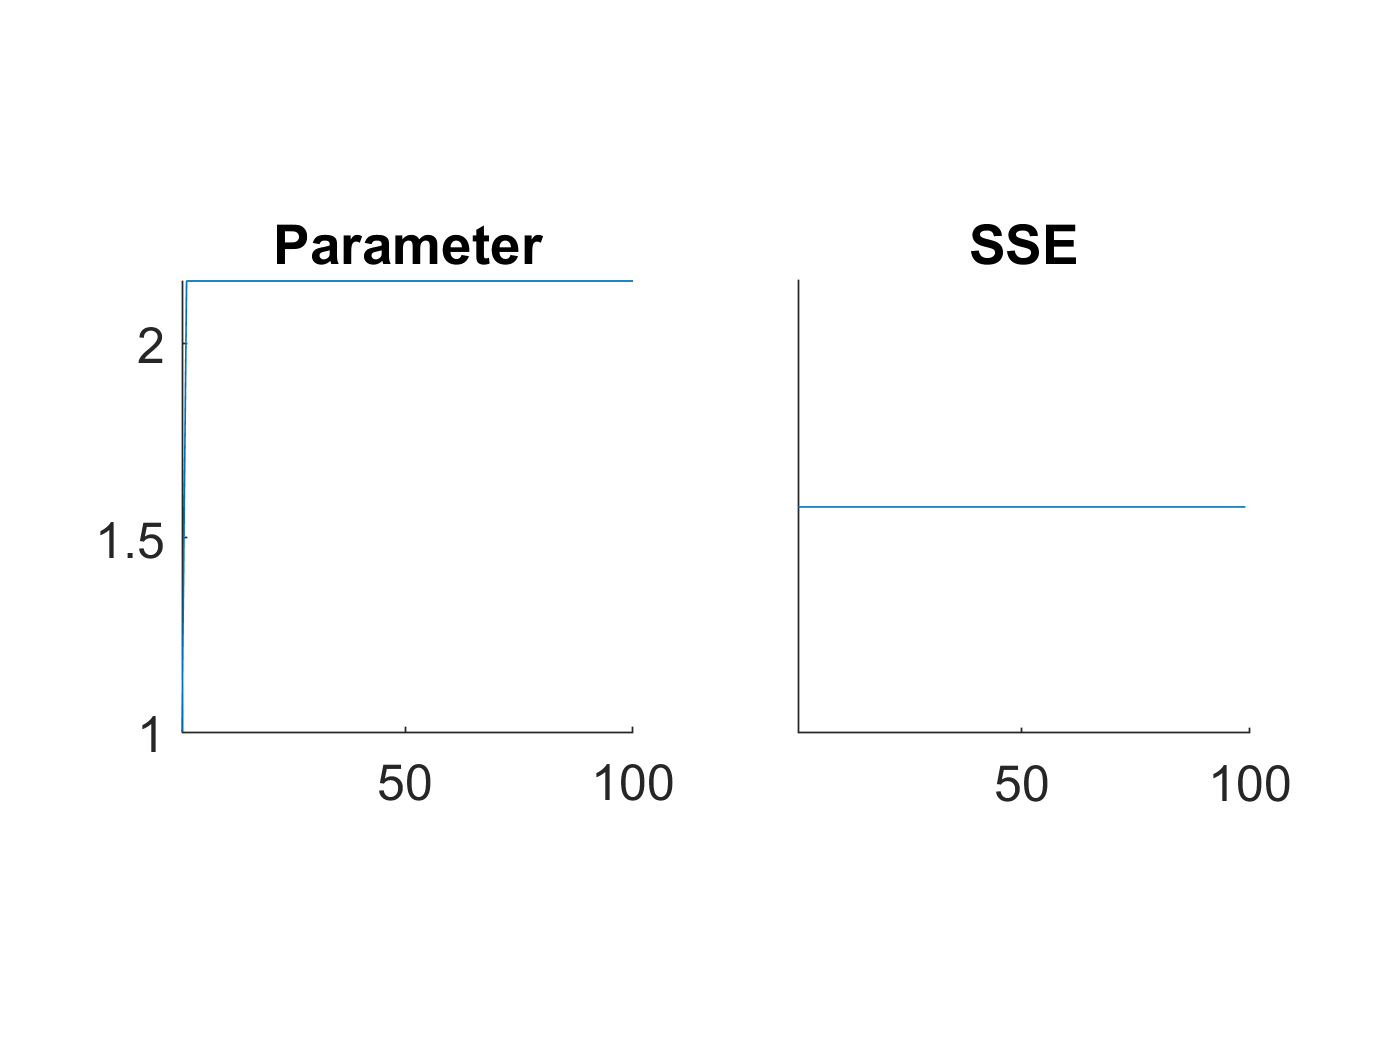
\includegraphics[scale=0.25]{figures/p_b_conv_1.png}
\end{figure}
}

\frame{
\frametitle{Gradient Matching with Smoothing}
We can also see how our model compares with the data:
\begin{figure}[H]
\centering
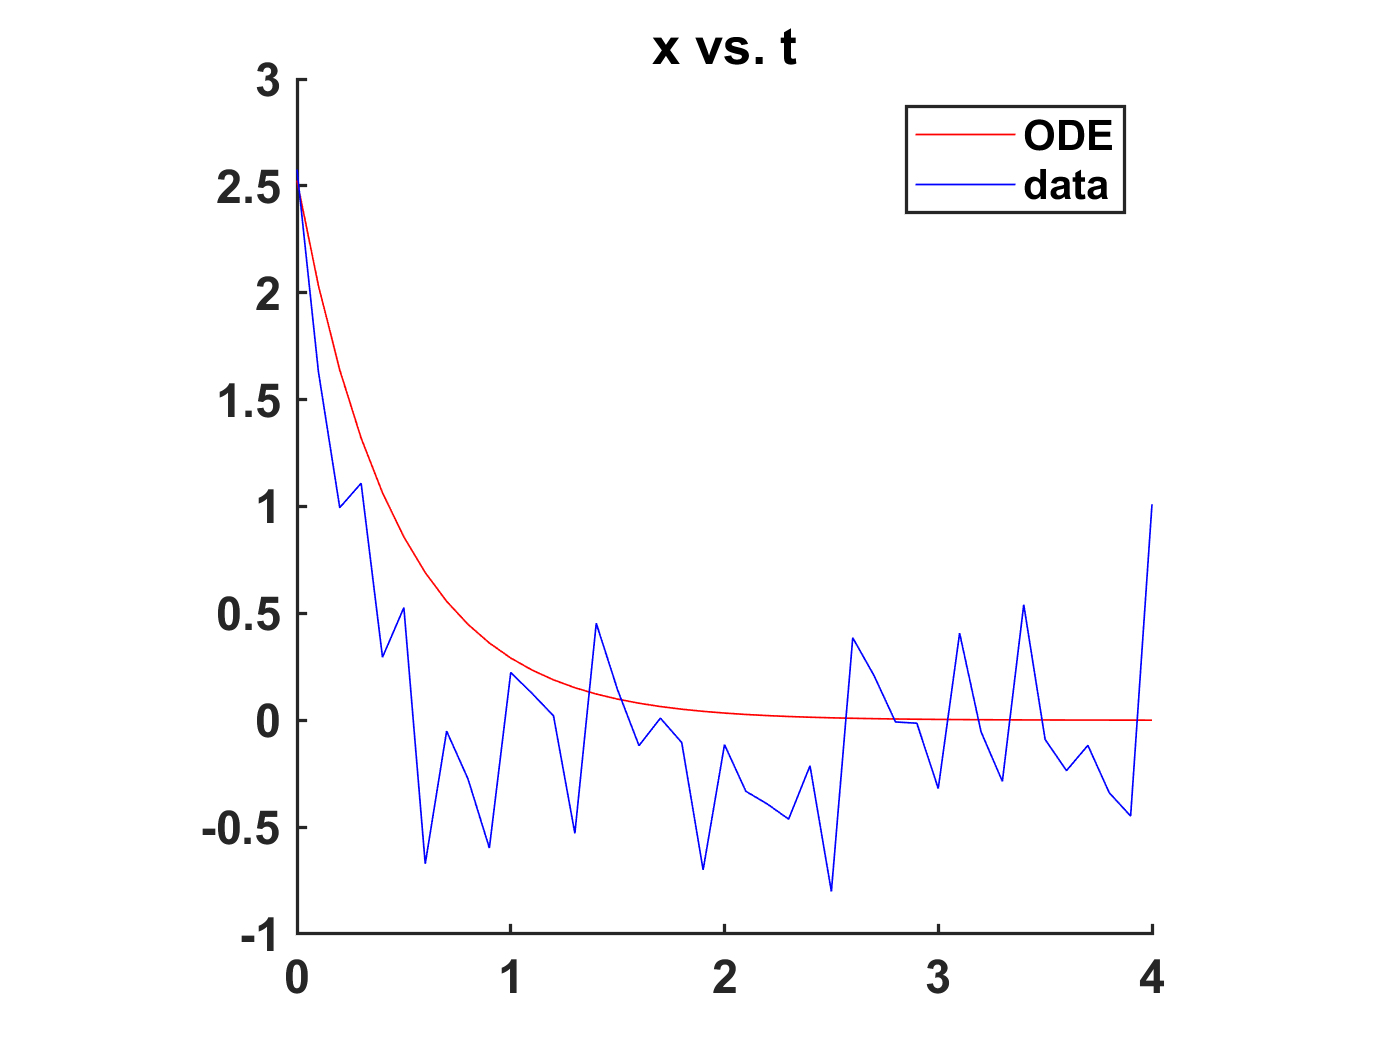
\includegraphics[scale=0.2]{figures/p_b_data_1.png}
\caption{The model we obtained is the line in blue. We can see that our model captures the trend of the data.}
\end{figure}
}

\frame{
\frametitle{Gradient Matching with Smoothing}
When the method is used without smoothing, it fails catastrophically. The parameter blows up.
}

\frame{
\frametitle{Gradient Matching with Smoothing}
When we smooth the data with collocations, we try different number of polynomials allowed for the basis and obtained the following result:\\
\begin{center}
\begin{tabular}{|c|c|}
\hline
Number of Polynomials & $\beta$\\
\hline
9 & 4.97277486579170\\
10 & 4.94682728787471\\
11 & 4.96241041092927\\
12 & 4.96995381483431\\
13 & 4.97336941885107\\
\hline
\end{tabular}
\end{center}
Therefore, the number of polynomials in the collocation basis does not affect the results drastically. 
}

\frame{
\frametitle{Integral Matching with Smoothing}

}

\frame{
\frametitle{Parameter Cascading with Smoothing}

}


\end{document}
